\documentclass{article}
\usepackage[a4paper, left=0.5in, right=0.5in, top=0.5in, bottom=0.5in]{geometry}
\usepackage{xcolor}
\usepackage{float}
\usepackage{graphicx}
\usepackage{xparse} % NewDocumentCommand, IfValueTF, IFBooleanTF

\usepackage{hyperref}
\usepackage{minted}

\usepackage{tikz-timing}[2014/10/29]
\usetikztiminglibrary[rising arrows]{clockarrows}

\NewDocumentCommand{\busref}{som}{\texttt{%
		#3%
		\IfValueTF{#2}{[#2]}{}%
		\IfBooleanTF{#1}{\#}{}%
}}

\newcommand{\chFormat}[1]{\emph{\textcolor{cyan}{#1}}}
\newcommand{\AXISignals}[1]{\textbf{\textcolor{magenta}{#1}}}

\title{AMBA AXI}
\author{Narendiran}
\date{\today}

\begin{document}
\large
    \maketitle

\quad AXI - Advacned eXtensible Interface
\subsubsection{Objectives}
\begin{itemize}
    \item high-performance, high frequency system for high-speed submicron interconnect
    \item high-bandwidth, low-latency
    \item flexibility in implementation of interconnect architecture
    \item backward-compatible with AHB and APB Interface
\end{itemize}
\subsubsection{Features}
\begin{itemize}
    \item seperate address/control and data phases
    \item unaligned data transfers using byte strobes
    \item burst-based transactions
    \item seperate read and write data channels to enabled low-cost DMA
    \item issue multiple outstanding addressess
    \item out-of-order transaction completion
    \item easy addition of register stages to provide timing closure
\end{itemize}

\section{Architecture}
\begin{itemize}
    \item AXI protocol is \emph{burst-based}.
    \item Every transaction has address and control information on the address channel which describes the nature of data transfers
    \item Data is transferred between master and slave
    \begin{itemize}
        \item Using a write data channel to the slave
        \item Using a read data channel to the master
    \end{itemize}
    \item In write transaction, all data flows from master to slave
    \item In write response channel, the slave signals the completion of write transaction to master.
\end{itemize}
\quad The read transaction can be seen below which uses \chFormat{Read address} and \chFormat{Read data} channel
\begin{figure}[H]
    \centering
    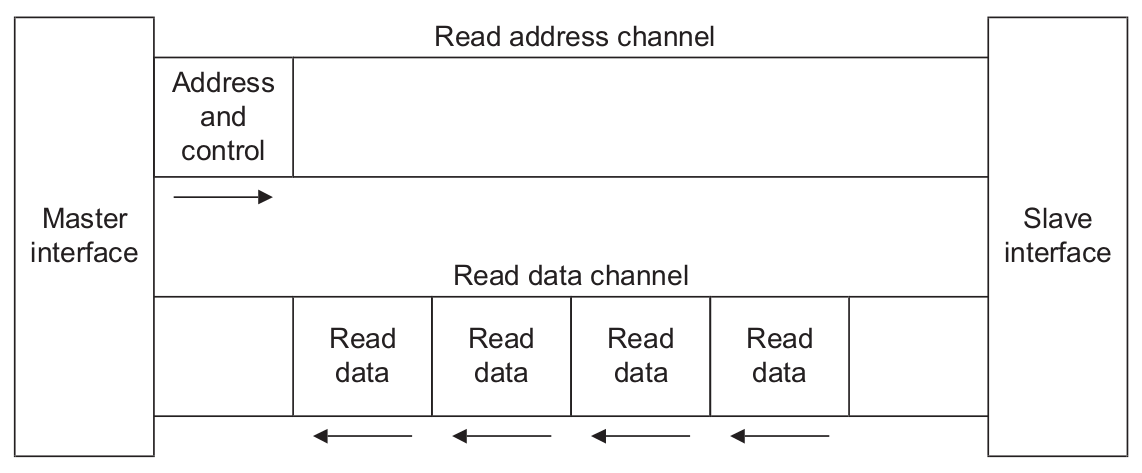
\includegraphics[width=1\textwidth]{Resources/ReadTransaction.png}
    \caption{Read transaction}
\end{figure}

\quad The write transaction can be seen below which uses \chFormat{Write address}, \chFormat{Write Data} and \chFormat{Write Response} channel
\begin{figure}[H]
    \centering
    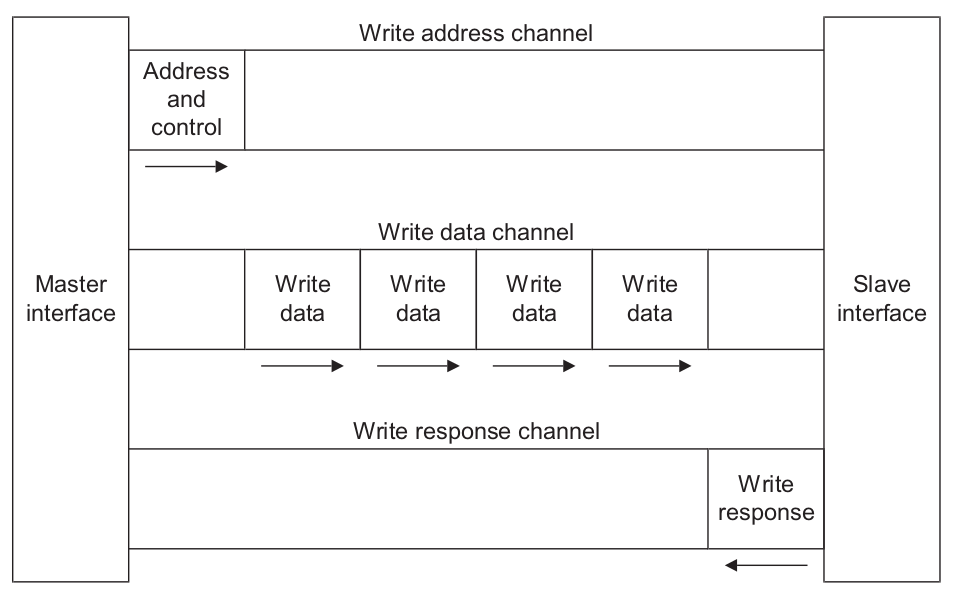
\includegraphics[width=1\textwidth]{Resources/WriteTransaction.png}
    \caption{Write transaction}
\end{figure}

\subsection{Channel Definition}
\begin{itemize}
    \item There are five channels namely \chFormat{Read Address} channel, \chFormat{Read Data} channel, \chFormat{Write Address} channel,\chFormat{Write Data} channel and \chFormat{Write Response} channel.
    \item All the five independent channels uses a two-way \AXISignals{VALID} and \AXISignals{READY} handshake mechanism.
    \begin{itemize}        
        \item The information Source uses the \AXISignals{VALID} signal to shown when valid data or control information is available on the channel.
        \item The Destination uses the \AXISignals{READY} signal to show it can accept the data.
    \end{itemize}
    \item The \chFormat{Read data} and \chFormat{Write data} channel uses the \AXISignals{LAST} signal to indicate the transfer of final data item withing a transaction.   
\end{itemize}
\subsubsection{Supported Mechanisms}
\begin{itemize}
    \item Variable-length bursts from 1 to 16 data transfers per burst.
    \item Each data transfer can have a transfer size 8 to 1024 bits.
    \item Gives ID tag to every transaction across interface.
    \item wrapping, incrementing and non-incrementing burts.
    \item atopic operations  using exclusive or locked accesses
    \item system-level caching and buffering control
    \item secure and priviledged access.
\end{itemize}

\subsubsection{Read Address Channel}
\begin{itemize}
    \item Read Tranaction has it's own address channel.
    \item Carries the required address and control information for the read transaction.
\end{itemize}

\subsubsection{Read Data Channel}
\begin{itemize}
    \item \chFormat{Read Data} channel conveys both read data and read response information from slave back to master.
    \item includes a data data bus which can be 8, 16, 32, 64, 128, 256, 512, 1024 bit width
    \item read response indicating the completion of read transaction.
\end{itemize}

\subsubsection{Write Address Channel}
\begin{itemize}
    \item Write Tranaction has it's own address channel.
    \item Carries the required address and control information for the write transaction.
\end{itemize}

\subsubsection{Write Data Channel}
\begin{itemize}
    \item \chFormat{Write data} channels conveys the write data from master to slave.
    \item include a data data bus which can be 8, 16, 32, 64, 128, 256, 512, 1024 bit width
    \item include one byte(8-bit) lane strobe for every eight data bits indicate which bytes of data bus are valid.
    \item \chFormat{Write data} channel information is buffered, so master can perfrom wirte transaction without slave acknowledgemnt of previous write transaction.
\end{itemize}

\subsubsection{Write Response Channel}
\begin{itemize}
    \item \chFormat{Write Response} channel proives a way for the slave to respond to write transactions
    \item All write transaction uses completion signalling.
    \item The completion signalling occurs once for each burst and not for each individual data transfer within a burst.
\end{itemize}


\subsection{Interface and Interconnect}
\quad Consist of master and slave devices connected together fthrough some interconnect.
\begin{figure}[H]
    \centering
    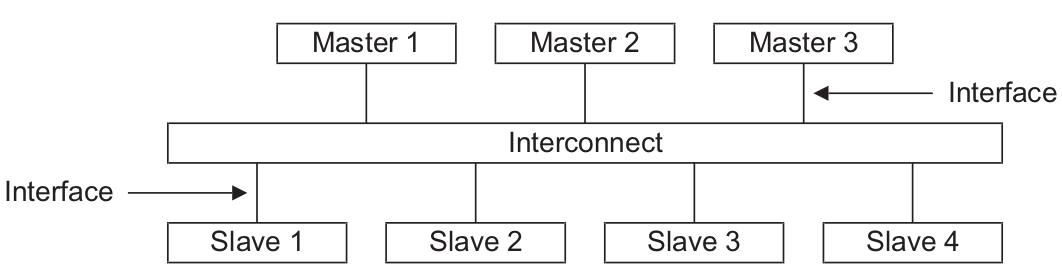
\includegraphics[width=1\textwidth]{./Resources/interconnect.png}    
    \caption{Interconnects}
\end{figure}

\subsection{Register Slices}
\begin{itemize}
    \item Each AXI channel transfer information in only one direction.
    \item Enables insertion of register slices in any channel at the cost of additional cycle of latency.
    \item Register slices can be used at any point within a interconnect.
\end{itemize}

\subsection{Read Burst example}
\quad THe following describes the read burst of four transfer.
\begin{figure}[H]
    \centering
    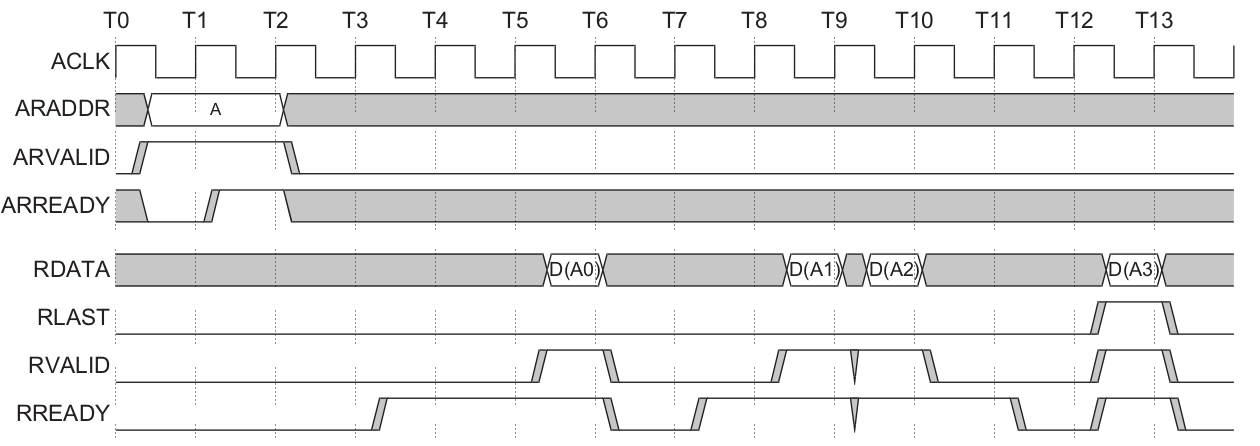
\includegraphics[width=1\textwidth]{./Resources/readBurstExample.png}    
    \caption{Read Burst Example}
\end{figure}
\begin{itemize}
    \item The \chFormat{read address} and \chFormat{read data} channels are used for this read transaction.
    \item Master drives the address and slave accept in one cycle.
    \begin{itemize}
        \item Master places the address on \AXISignals{ARADDR} bus in the \chFormat{read address} channel.
        \item Master makes the \AXISignals{ARVALID} HIGH to indicate that read address is available and its valid.
        \item Then, the slave makes the \AXISignals{ARREADY} signal HIGH to indicate its ready to accept the address
    \end{itemize} 
    \item The master on receiving the \AXISignals{ARREADY} signal of the \chFormat{read address} channel from the slave, makes the \AXISignals{RREADY} signal of the \chFormat{Read data} channel HIGH.
    \item Now, the slave sends the data throught the \chFormat{read data} channels.
    \begin{itemize}
        \item Slave places the data on to the \AXISignals{RDATA} bus and makes the \AXISignals{RVALID} signal HIGH to start the data transfer.
        \item Now, the master on receives the first data by checking the \AXISignals{RVALID} signal form the slave.
        \item On receiving the data, the master makes the \AXISignals{RREADY} signal LOW untill it can process the recieved data from slave.
        \item WHen master is ready to receive, the master makes the \AXISignals{RREADY} singal HIGH to indicate it can receive further data.
    \end{itemize}
    \item Now, the slave places the second data onto the \AXISignals{RDATA} bus and makes the \AXISignals{RVALID} signal HIGH.
    \item The above process repeates.
    \item When the last data is to be sent, the slave placess the last data onto the \AXISignals{RDATA} bus and makes the \AXISignals{RLAST} and \AXISignals{RVALID} HIGH.
\end{itemize}


\subsection{Overlapping read example}
\begin{itemize}
    \item Master drives another burst address after slave accpets the first address.
    \item this enables the slave to begin processing data for second burst in parallel with completion of first bus.
    \item The following describes the Overlapping read burst example.
\end{itemize}
\begin{figure}[H]
    \centering
    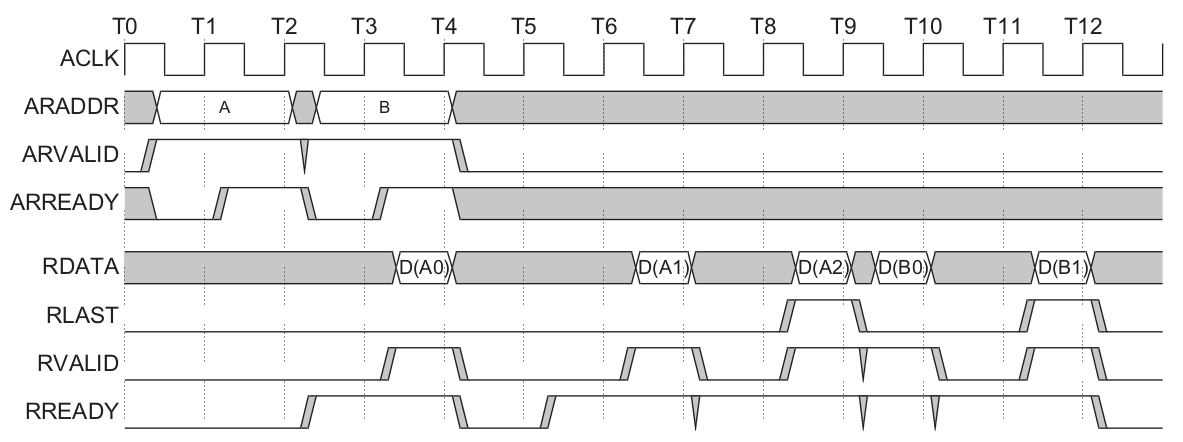
\includegraphics[width=1\textwidth]{./Resources/overlappingBurstExample.png}    
    \caption{Overlapping Burst Example}
\end{figure}

\begin{itemize}
    \item The \chFormat{read address} and \chFormat{read data} channels are used for this read transaction.
    \item Master drives the address and slave accept in one cycle.
    \begin{itemize}
        \item Master places the address on \AXISignals{ARADDR} bus in the \chFormat{read address} channel.
        \item Master makes the \AXISignals{ARVALID} HIGH to indicate that read address is available and its valid.
        \item Then, the slave makes the \AXISignals{ARREADY} signal HIGH to indicate its ready to accept the address
    \end{itemize} 
    \item The master on receiving the \AXISignals{ARREADY} signal of the \chFormat{read address} channel from the slave, makes the \AXISignals{RREADY} signal of the \chFormat{Read data} channel HIGH.
    \item Now, the slave sends the data throught the \chFormat{read data} channels.
    \item During the above process, the master places the next address to be read for next read burst onto the \AXISignals{ARADDR} bus and makes the \AXISignals{ARVALID} singal.
    \item Now, the slave along with responding to the previous read transaction, it makes the \AXISignals{ARREAD} HIGHT to indicate it can receive data.
    \item As soon as the slave completes the first data transaction, the slave begins the next transaction by placing the data onto \AXISignals{RDATA} bus and making the \AXISignals{RVALID} singal HIGH.
\end{itemize}

\subsection{Write Burst example}
\quad The following describes the write burst example.
\begin{figure}[H]
    \centering
    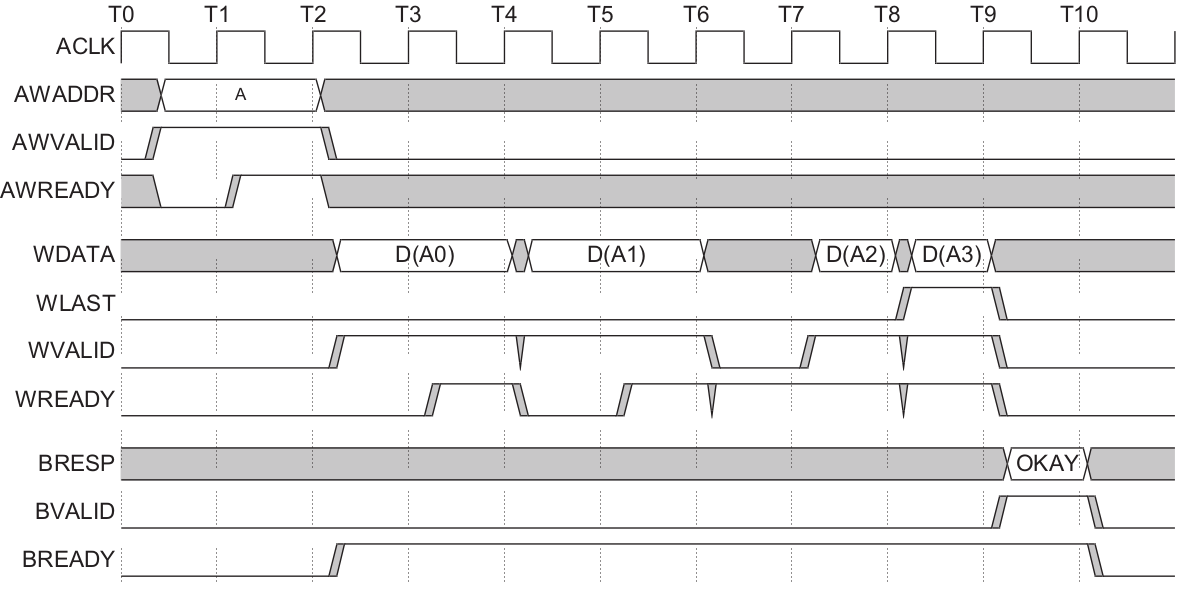
\includegraphics[width=1\textwidth]{./Resources/writeBurstExample.png}    
    \caption{Write Burst Example}
\end{figure}
\begin{itemize}
    \item The \chFormat{Write address}, \chFormat{Write Data} and \chFormat{Write Response} channel are used for this write transaction.
    \item The process is started by master placing the address and control information onto the \chFormat{write address} channel.
    \begin{itemize}
        \item Master places the address onto the \AXISignals{AWADDR} bus and mkes the \AXISignals{AWVALID} singal HIGH.
        \item Now, the slaves accepts the address from master after one cycle by making the \AXISignals{AWREAD} signal HIGH.
    \end{itemize}
    \item Also, the master makes the \AXISignals{BREADY} singal HIGH in the \chFormat{write response} channel for getting the response of this write transaction.
    \item After the slave responds by making the \AXISignals{AWREADY} HIGHT, the master starts sending the data and control information in the \chFormat{write data} channel.
    \begin{itemize}
        \item THe master places the first data to be sent onto to the \AXISignals{WDATA} bus and makes the \AXISignals{WVALID} signal HIGH.
        \item After one cycle, the slave accepts the data from master by making the \AXISignals{WREADY} signal HIGH.
        \item After accepting the data, the slave mkaes the \AXISignals{WREADY} singal LOW for processing.        
    \end{itemize} 
    \item Now, the master sends the next data onto the \AXISignals{WDATA} bus and makes the \AXISignals{WVALID} singal HIGH.
    \item The above process is repeated for further data.
    \item When sending the last data, the master places the data onto the \AXISignals{WDATA} bus and makes the \AXISignals{WVALID} singal and \AXISignals{WLAST} singal HIGH.
    \item The slave makes the \AXISignals{WREADY} for the last time for that write transaction and accepts the data.
    \item Now, the slave responds to master by driving the \chFormat{Write Response} channel to indicate the completion of write transaction.
    \begin{itemize}
        \item The slave makes the \AXISignals{BRESP} signal to be \emph{\textcolor{green}{OKAY}} to indicate the success and makes the \AXISignals{BVALID} singal HIGH.
    \end{itemize}
\end{itemize}

\section{Signal Description}
\subsection{Global Signals}
\begin{itemize}
    \item \AXISignals{ACLK} - Global AXI clock - All signals are sampled at rising edge of this Global clock.
    \item \AXISignals{ARESETn} - GLobal Reset - Active LOW global reset.
\end{itemize}

\subsection{Write Address channel}
\begin{table}[H]
    \begin{center}
        \begin{tabular}{c|c|c|p{9.5cm}}
            \textbf{Signals} & \textbf{Source} & \textbf{Name} & \textbf{Description}\\
            \hline
            AWID[3:0] & Master & Write Address ID & ID tag for write address group of signal.\\
            AWADDR[31:0] & Master & Write Address & The actual write address for first transfer in a write burst transaction.\\
            AWLEN[3:0] & Master & Burst length & Number of data transfers in a burst associated with address.\\
            AWSIZE[2:0] & Master & Burst size & Size of each data transfer in a burst.\\
            AWBURST[1:0] & Master & Burst Type & Burst type along with size information calculates addresses for each transfer withing burst.\\
            AWLOCK[1:0] & Master & Lock Type & Atomic Characteristics of transfer.\\
            AWCACHE[3:0] & Master & Cache Type & indicates the bufferable, cacheable, write-through, write-back and allocate attributes of the transaction.\\
            AWPROT[2:0] & Master & Projection Type & indicates the normal, privileged, or secure protection level of the transaction and whether the transaction is a data access or an instruction access.\\
            AWVALID & Master & Write address valid & 1 - address and control information are available and valid. Address and control information should be stable until address acknowledgemnt signal \AXISignals{AWREADY} goes HIGH.\\
            AWREADY & Slave & Write address ready & 1 - salve ready to accept an address and associated control signal.\\
        \end{tabular}
    \end{center}
\end{table}

\subsection{Write Data channel}
\begin{table}[H]
    \begin{center}
        \begin{tabular}{c|c|c|p{9.5cm}}
            \textbf{Signals} & \textbf{Source} & \textbf{Name} & \textbf{Description}\\
            \hline
            WID[3:0] & Master & Write ID & ID tag for write data group of signal. \AXISignals{WID} must be equal to \AXISignals{AWID} for write transaction.\\
            WDATA[31:0] & Master & Write Data & The actual write data. Can be 8, 16, 32, 64, 128, 256, 512 or 1024 bits wide\\
            WSTRB[3:0] & Master & Write Strobes & indicates which byte lanes to update in memory. One write strobe for each eight bits of write data bus.
            \begin{center}
                $WSTRB[n] = WDATA[(8*n) + 7:(8*n)]$
            \end{center}\\
            WLAST & Master & Write last & indicate the last data transfer in a write burst.\\
            WVALID & Master & Write valid & 1 - write data and stobes are available and valid.\\
            WREADY & Slave & Write ready & 1 - salve ready to accept write data.\\
        \end{tabular}
    \end{center}
\end{table}

\subsection{Write Response channel}
\begin{table}[H]
    \begin{center}
        \begin{tabular}{c|c|c|p{9.5cm}}
            \textbf{Signals} & \textbf{Source} & \textbf{Name} & \textbf{Description}\\
            \hline
            BID[3:0] & Slave & Response ID & ID tag for write response group of signal. \AXISignals{BID} must be equal to \AXISignals{AWID} for write transaction.\\
            BRESP[1:0] & Slave & Write Response & indicates the status of write transaction and can take \emph{\textcolor{green}{OKAY}}, \emph{\textcolor{green}{EXOKAY}}, \emph{\textcolor{green}{SLVERR}} and \emph{\textcolor{green}{DECERR}}.\\
            BVALID & Slave & Write responds valid & 1 - write response is available and valid.\\
            BREADY & Master & Write response ready & 1 - master ready to accept response information.\\
        \end{tabular}
    \end{center}
\end{table}

\subsection{Read Address channel}
\begin{table}[H]
    \begin{center}
        \begin{tabular}{c|c|c|p{9.5cm}}
            \textbf{Signals} & \textbf{Source} & \textbf{Name} & \textbf{Description}\\
            \hline
            ARID[3:0] & Master & Read address ID & ID tag for read address group of signal.\\
            ARADDR[31:0] & Master & Read Address & The actual read address for first transfer in a read burst transaction.\\
            ARLEN[3:0] & Master & Burst length & Number of data transfers in a burst associated with address.\\
            ARSIZE[2:0] & Master & Burst size & Size of each data transfer in a burst.\\
            ARBURST[1:0] & Master & Burst Type & Burst type along with size information calculates addresses for each transfer within burst.\\
            ARLOCK[1:0] & Master & Lock Type & Atomic Characteristics of transfer.\\
            ARCACHE[3:0] & Master & Cache Type & indicates cacheable attributes of the transaction.\\
            ARPROT[2:0] & Master & Projection Type & indicates the protection unit information transaction.\\
            ARVALID & Master & Read address valid & 1 - address and control information are available and valid. Address and control information should be stable until address acknowledgemnt signal \AXISignals{ARREADY} goes HIGH.\\
            ARREADY & Slave & Read address ready & 1 - salve ready to accept an address and associated control signal.\\
        \end{tabular}
    \end{center}
\end{table}

\subsection{Read Data channel}
\begin{table}[H]
    \begin{center}
        \begin{tabular}{c|c|c|p{9.5cm}}
            \textbf{Signals} & \textbf{Source} & \textbf{Name} & \textbf{Description}\\
            \hline
            RID[3:0] & Slave & Read ID & ID tag for read data group of signal. \AXISignals{RID} must be equal to \AXISignals{ARID} for read transaction.\\
            RDATA[31:0] & Slave & Read Data & The actual read data. Can be 8, 16, 32, 64, 128, 256, 512 or 1024 bits wide\\
            RRESP[1:0] & Slave & Read Response & indicate the status of read transfer and can be  \emph{\textcolor{green}{OKAY}}, \emph{\textcolor{green}{EXOKAY}}, \emph{\textcolor{green}{SLVERR}} and \emph{\textcolor{green}{DECERR}}.\\
            RLAST & Slave & Read last & indicate the last data transfer in a read burst.\\
            RVALID & Slave & Read valid & 1 - read data are available and valid.  read transfer is complete \\
            RREADY & Master & Read ready & 1 - master ready to accept read data and response information.\\
        \end{tabular}
    \end{center}
\end{table}

\section{Channel Handshake}
\subsection{Handshake Procedure}
\begin{itemize}
    \item All five channels use the \AXISignals{VALID} and \AXISignals{READY} singal for handshaking.
    \item Control the rate at which data and control information moves.
    \item The source generates the \AXISignals{VALID} signal indicating the data or control information is available.
    \item The Destination generates the \AXISignals{READY} singal indicating that it can accept the data or control information.
    \item \textbf{Transfer occurs only when both \AXISignals{VALID} and \AXISignals{READY} signals are HIGH.}
\end{itemize}

\subsubsection{Example Handshake sequence}
\subsubsection*{VALID before READY}
\begin{figure}[H]
    \centering
    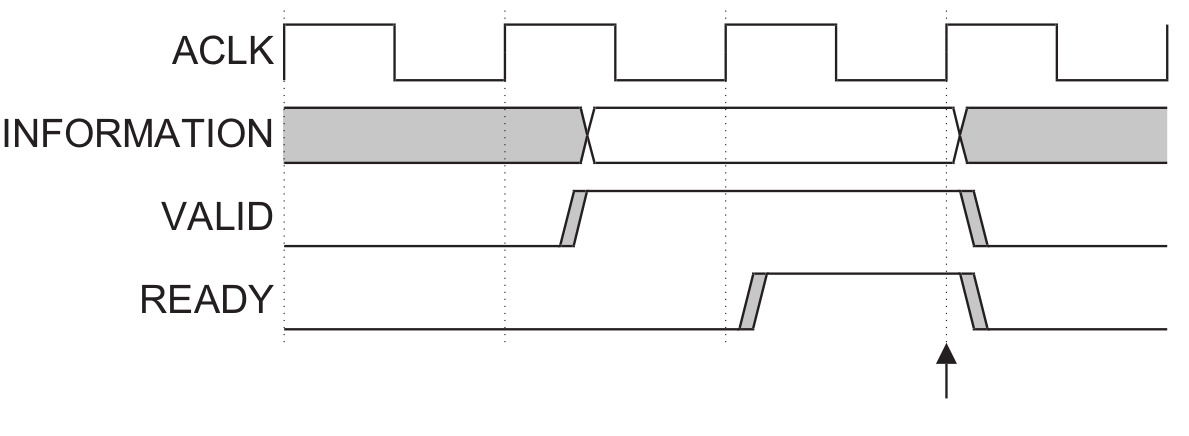
\includegraphics[width=1\textwidth]{Resources/ValidBeforeReady.png}
    \caption{VALID before READY}
\end{figure}
\begin{itemize}
    \item The source presents the data or control information and drives the \AXISignals{VALID} signal HIGH.
    \item The data or control information from the source remains stable until the destination drives the READY signal HIGH, indicating that it accepts the data or control information.
    \item The arrow shows when the transfer occurs.
\end{itemize}

\subsubsection*{READY before VALID}
\begin{figure}[H]
    \centering
    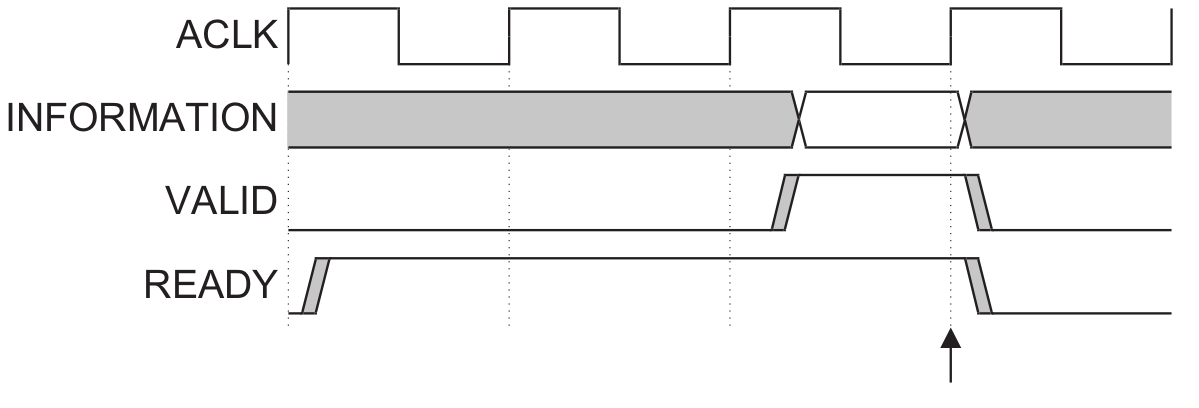
\includegraphics[width=1\textwidth]{Resources/ReadyBeforeValid.png}
    \caption{VALID before READY}
\end{figure}
\begin{itemize}
    \item The destination drives \AXISignals{READY} HIGH before the data or control information is valid.
    \item This indicates that destination can accept data or control information in a sigle cyle as soon as it becomes valid.
    \item The arrow shows when the transfer occurs.
\end{itemize}

\subsubsection*{VALID with READY}
\begin{figure}[H]
    \centering
    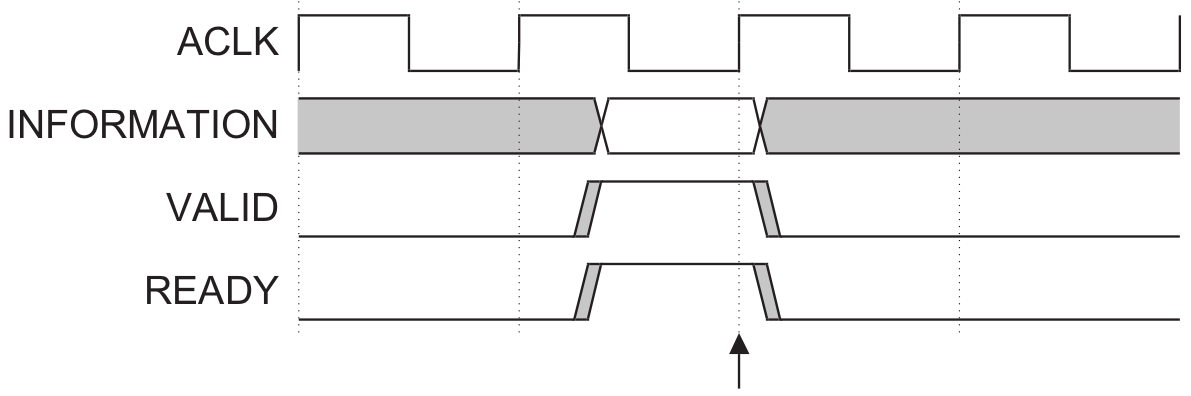
\includegraphics[width=1\textwidth]{Resources/ReadyWithValid.png}
    \caption{VALID before READY}
\end{figure}
\begin{itemize}
    \item Both the source and destination happns to indicate in same cycle that they can transfer data or control information.
    \item The transfer occurs immediately.
    \item The arrow shows when the transfer occurs.
\end{itemize}
\textbf{Notes: }In all the above cases, we can see the \AXISignals{VALID}  is made high only when data is valide.

\subsection{Write Address Channel}
\begin{itemize}
    \item Master places the valid addresses and control information and makes the \AXISignals{AWVALID} singal HIGH.
    \item The address and control information and \AXISignals{AWVALID} remains in that statue until slave accepts the address and control information.
    \item Now the salve makes the \AXISignals{AWREADY} singal HIGH.
\end{itemize}
\begin{tikztimingtable}[%
    timing/dslope=0.1,
    timing/.style={x=5ex,y=2ex},
    x=5ex,
    timing/rowdist=3ex,
    timing/name/.style={font=\sffamily\scriptsize}
    ]
    \busref{ACLK}  & [C] C C C C C 12{C}\\
    \busref{AWADDR}  & U U U 3D{Valid Address}  U U  U U  U UU  U U  U U \\
    \busref{AWVALID} & L LL HHH LLLLLLLLLLL\\
    \busref{AWREADY} & UUULH H UUUUUUUUUUU\\
\end{tikztimingtable}

\textbf{Note: } The default value for \AXISignals{AWREADY} should be HIGH.

\subsection{Write Data channel}
\begin{itemize}
    \item Master places the valid write data and makes the \AXISignals{WVALID} signal HIGH.
    \item This \AXISignals{WVALID} singal must remain in that state untill the slave accepts the write data and makes the \AXISignals{WREADY} singal HIGH.
    \item The master must drive \AXISignals{WLAST} singal HIGH when writing the final write data transfer in a burst.
    \item When the \AXISignals{WVALID} is LOW, \AXISignals{WSTRB[3:0]} must be LOW or held at previous value.
\end{itemize}
\begin{tikztimingtable}[%
    timing/dslope=0.1,
    timing/.style={x=5ex,y=2ex},
    x=5ex,
    timing/rowdist=3ex,
    timing/name/.style={font=\sffamily\scriptsize}
    ]
    \busref{ACLK}  & [C] C C C C C 12{C}\\
    \busref{WDATA}  & U U U 3D{Valid Data}  U U  U U  U UU  U U  U U \\
    \busref{WVALID} & L LL HHH LLLLLLLLLLL\\
    \busref{WREADY} & UUULH H UUUUUUUUUUU\\
\end{tikztimingtable}

\textbf{Note: } The default value for \AXISignals{WREADY} should be HIGH only if the slave can always accept write data in a single cycle.


\subsection{Write Response channel}
\begin{itemize}
    \item Slave makes the \AXISignals{BVALID} singal HIGH when it drives the valid write response.
    \item \AXISignals{BVALID} must be HIGH until the master accpets the response and asserts the \AXISignals{BREADY} singal.
    \item The default value of \AXISignals{BREADY} is HIGH only if master can always accept the write response in a single cycle.
\end{itemize}
\begin{tikztimingtable}[%
    timing/dslope=0.1,
    timing/.style={x=5ex,y=2ex},
    x=5ex,
    timing/rowdist=3ex,
    timing/name/.style={font=\sffamily\scriptsize}
    ]
    \busref{ACLK}  & [C] C C C C C 12{C}\\
    \busref{BRESP}  & 12{U} 2D{OKAY}  U U  U \\
    \busref{BVALID} & 12{L} HH LL L\\
    \busref{BREADY} & LLLLLL HHHHHHHH LLL\\
\end{tikztimingtable}

\subsection{Read Data channel}
\begin{itemize}
    \item Slave places the valid read data and makes the \AXISignals{RVALID} signal HIGH.
    \item This \AXISignals{RVALID} singal must remain in that state untill the master accepts the read data and makes the \AXISignals{RREADY} singal HIGH.
    \item The slave must drive \AXISignals{RLAST} singal HIGH indicating that its transferig the last data transfer in the read burst.
\end{itemize}
\begin{tikztimingtable}[%
    timing/dslope=0.1,
    timing/.style={x=5ex,y=2ex},
    x=5ex,
    timing/rowdist=3ex,
    timing/name/.style={font=\sffamily\scriptsize}
    ]
    \busref{ACLK}  & [C] C C C C C 12{C}\\
    \busref{RDATA}  & U U U 3D{Valid Data}  U U  U U  U UU  U U  U U \\
    \busref{RVALID} & L LL HHH LLLLLLLLLLL\\
    \busref{RREADY} & UUULH H UUUUUUUUUUU\\
\end{tikztimingtable}

\textbf{Note: } The default value for \AXISignals{RREADY} should be HIGH only if the master can always accept the read data immediately..

\subsection{Relationship of handshake signals among channels}
\begin{itemize}
    \item Make \AXISignals{READY} signal HIGH before \AXISignals{VALID} for better efficiency.
    \item The single-headed arrow point to signal that can be asserted before or after the previous signal.
    \item The double-headed arrow point to signal that must be asserted only after the previous signal.
    \item For read transaction,
\begin{figure}[H]
    \centering
    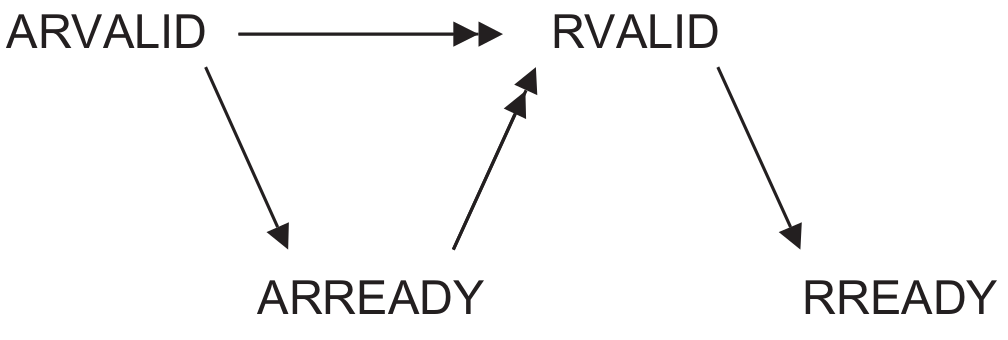
\includegraphics[width=0.5\textwidth]{Resources/ReadtransactionHandshakeDependencies.png}
    \caption{Read transaction handshake dependencies}
\end{figure}
    \item the slave can wait for \AXISignals{ARVALID} to be asserted before it asserts \AXISignals{ARREADY} singal.
    \item the slave must wait for both \AXISignals{ARVALID} and \AXISignals{ARREADY} to be asserted befoere it starts to return data by asserting \AXISignals{RVALID}.
    \item For Write transaction,
    \begin{figure}[H]
        \centering
        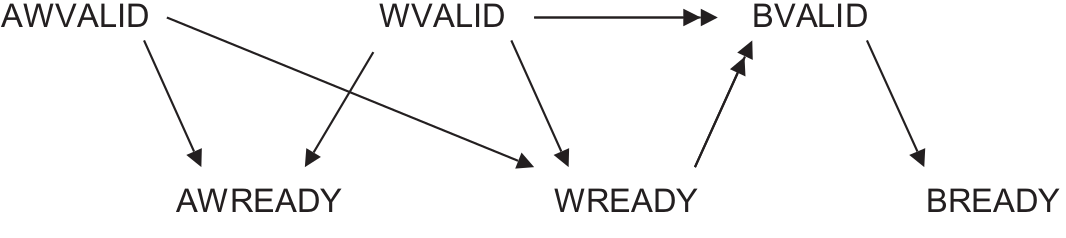
\includegraphics[width=0.5\textwidth]{Resources/WritetransactionHandshakeDependencies.png}
        \caption{Write transaction handshake dependencies}
    \end{figure}
    \item the master must not wait for the slave to assert \AXISignals{AWREADY} or \AXISignals{WREADY} before asserting \AXISignals{AWVALID} or \AXISignals{WVALID}
    \item the slave can wait for \AXISignals{AWVALID} or \AXISignals{WVALID}, or both, before asserting \AXISignals{AWREADY} and/or \AXISignals{WREADY}
    \item the slave must wait for both \AXISignals{WVALID} and \AXISignals{WREADY} to be asserted before asserting \AXISignals{BVALID}
\end{itemize}

\section{Addressing Options}
\begin{itemize}
    \item AXI protocol is burst-based.
    \item THe master begin each burst by driving transfer control information and address of the first byte in the transfer.
    \item As the burst progresses, the slave must calculate the address of subsequent transfers in the burst.
    \item Burst must not cross 4KB boundaries.
\end{itemize}

\subsection{Burst Length}
\begin{itemize}
    \item The \AXISignals{AWLEN} or \AXISignals{ARLEN} singal specifies the Number of data transfer withing each burst.
    \item The \AXISignals{AWLEN} or \AXISignals{ARLEN} singal can take values between 1(4'b0000) to 16(4'b1111).
\end{itemize}

\subsection{Burst Size}
\begin{itemize}
    \item The \AXISignals{AWSIZE} or \AXISignals{ARSIZE} singal specifies the Number of data bytes in each beat or data transfer.
    \item The \AXISignals{AWSIZE} or \AXISignals{ARSIZE} singal can take values as shown
       
    \begin{center}
        \begin{tabular}{c|c}
            \textbf{ARSIZE[2:0]} or \textbf{AWSIZE[2:0]} & \textbf{Bytes in each transfer}\\
            \hline
            3'b000 & 1\\
            3'b001 & 2\\
            3'b010 & 4\\
            3'b011 & 8\\
            3'b100 & 16\\
            3'b101 & 32\\
            3'b110 & 64\\
            3'b111 & 128\\
        \end{tabular}
    \end{center}
    \item AXI determines the trandfer address and also which byte lane to use.
\end{itemize}

\subsection{Burst Type}
\begin{table}[H]
    \begin{center}
        \begin{tabular}{c|c|p{2cm}|p{6.5cm}}
            \textbf{ARBURST[1:0] or AWBURST[1:0]} & \textbf{Burst type} & \textbf{Access} & \textbf{Descritpion}\\
            \hline
            2'b00 & FIXED & FIFO-type & Fixed-address burst -- address remains same for every data transfer in the burst; Used in case of repeated acesses to same location such as when loading or emptying  peripheral FIFO.\\
            2'b01 & INCR & Normal sequential memory & incrementing-address burst -- the address for each transfer in the burst in an increment of the previous transfer address. The incrementing value depends on the size of the transfer. If the burst size is 4, then the address of each transfer is previous address plus 4\\
            2'b10 & WRAP & Cache line & incrementing-address burst that wraps to a lower address at wratp boundaries -- wrap boundarry is the size of each transfer in burst multiplied by total number of transfer in the burst.\\
        \end{tabular}
    \end{center}
\end{table}

\subsection{Burst address}
\quad The Variables used are
\begin{itemize}
    \item \emph{Start\_Address} - Start address issued by the master.
    \item \emph{Numbe\_Bytes} - Maximum Number of bytes in each data transfer.
    \item \emph{Data\_Bus\_Bytes} - Number of byte lanes in the data bus.
    \item \emph{Aligned\_Addres} - Aligned version of start address.
    \item \emph{Burst\_Length} - total Number of data transfers within a burst.
    \item \emph{Address\_N} - address of transfer N within a burst.
    \item \emph{Wrap\_Boundary} - Lowest address withing a wrapping burst.
    \item \emph{Lower\_Byte\_Lane} - Byte lane of lowest addressed byte of a transfer.
    \item \emph{Upper\_Byte\_Lane} - Byte lane of highest addressed byte of a transfer.
    \item \emph{INT(x)} - Rounded-down integer value of x.
\end{itemize}

\begin{itemize}
    \item Addresses of tranfers within a burst
    \begin{itemize}
        \item[$*$] $Start\_Address = ADDR$
        \item[$*$] $Number\_Bytes = 2^{SIZE}$
        \item[$*$] $Burst\_Lenght = LEN + 1 $
        \item[$*$] $Aligned\_Address = INT(\frac{Start\_Address}{Number\_Bytes}) * Number\_Bytes$
    \end{itemize}
    \item First Address
    \begin{itemize}
        \item[$*$] $Address\_1 = Start\_Address$
    \end{itemize}
    \item Address of any tranfer after the first transfer in a burst
    \begin{itemize}
        \item[$*$] $Address\_N = Aligned\_Address + (N-1)*Number\_Bytes$
    \end{itemize}
    \item The wrapping boundary in wrapping burst
    \begin{itemize}
        \item[$*$] $Wrap\_Boundary = INT(\frac{Start\_Address}{Number\_Bytes * Burst\_Length}) * Number\_Bytes * Burst\_Length$ 
        \item[$*$] $Address\_N = Wrap\_Boundary$. 
    \end{itemize}
    \item Data is transferred on
    \begin{itemize}
        \item[$*$] $DATA[(8*Upper\_Byte\_Lane) + 7 : (8*Lower\_Byte\_Lane)]$
    \end{itemize}
\end{itemize}

\section{Basic Interface for Master}
\begin{minted}[style=perldoc]{verilog}
//Global Signals
input wire  M_AXI_ACLK,
input wire  M_AXI_ARESETN,
// Write address interface (issued by master)
output wire [32-1 : 0] M_AXI_AWADDR,
output wire [2 : 0] M_AXI_AWPROT,
output wire  M_AXI_AWVALID,
input wire  M_AXI_AWREADY,
// Write Data interface (issued by master)
output wire [32-1 : 0] M_AXI_WDATA,
output wire [32/8-1 : 0] M_AXI_WSTRB,
output wire  M_AXI_WVALID,
input wire  M_AXI_WREADY,
// Write Response interface (issued by slave)
input wire [1 : 0] M_AXI_BRESP,
input wire  M_AXI_BVALID,
output wire  M_AXI_BREADY,
// Read Address interface (issued by master)
output wire [32-1 : 0] M_AXI_ARADDR,
output wire [2 : 0] M_AXI_ARPROT,
output wire  M_AXI_ARVALID,
input wire  M_AXI_ARREADY,
// Read Data interface (issued by slave)
input wire [32-1 : 0] M_AXI_RDATA,
input wire [1 : 0] M_AXI_RRESP,
input wire  M_AXI_RVALID,
output wire  M_AXI_RREADY
\end{minted}
\section{AXI Single Read}
\begin{itemize}
    \item A single read using AXI protocol.
    \item Uses just the \chFormat{read address} and \chFormat{read data} channel.
    \item Manipulating the \AXISignals{AWADDR}, \AXISignals{ARVALID} and \AXISignals{RREADY} signals only.
    \item We read data from BRAM using AXI interface.
    \item Initial content of BRAM is the \href{./MemFiles/SampleMemFile.coe}{Sample Mem coe file}.
\end{itemize}
\subsection{Block Diagram}
\begin{figure}[H]
    \centering
    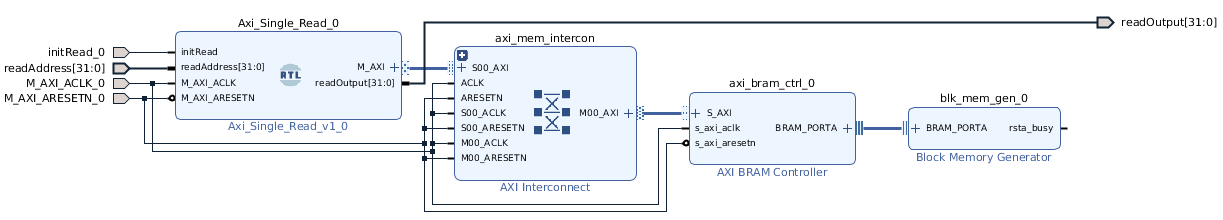
\includegraphics[width=1\textwidth]{Resources/SingleReadBRAM.png}
\end{figure}
\subsection{Code}
\begin{minted}[style=perldoc]{verilog}
// for ARVALID                                                                
always @(posedge M_AXI_ACLK)                                                     
    begin                                                                            
        if (M_AXI_ARESETN == 0)                                                       
          begin                                                                        
            axi_arvalid <= 1'b0;                                                       
          end     
        else if (init_txn_pulse == 1'b1)                                                    
          begin                                                                        
            axi_arvalid <= 1'b1;                                                       
          end         
        else if (M_AXI_ARREADY==1 && axi_arvalid==1)                                         
          begin                                                                        
            axi_arvalid <= 1'b0;                                                       
          end                                                                            
    end
    
// for RREADY
always @(posedge M_AXI_ACLK)                                    
    begin                                                                 
        if (M_AXI_ARESETN == 0)                                            
          begin                                                             
            axi_rready <= 1'b0;                                             
          end                                         
        else if (M_AXI_RVALID==1 && axi_rready==0)                               
          begin                                                             
            axi_rready <= 1'b1;                                             
          end                                                                
        else if (axi_rready==1)                                                
          begin                                                             
            axi_rready <= 1'b0;                                             
          end                                                               
    end 
    
// Reading the data
reg [31:0]myVal;
always @(posedge M_AXI_ACLK)                                                      
  begin                                                                             
    if (M_AXI_ARESETN == 0)                                                         
        myVal <= 1'b0;                                                     
    else if (M_AXI_RVALID==1 && axi_rready==1)         
      myVal <= M_AXI_RDATA;                                                        
    else                                                                            
      myVal <= myVal;                                               
  end 
\end{minted}

\subsection{Output}
\begin{figure}[H]
    \centering
    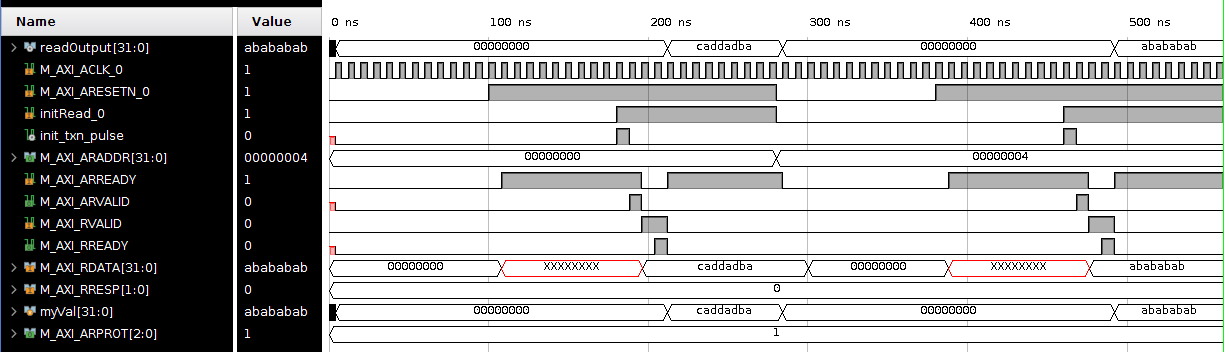
\includegraphics[width=1\textwidth]{Resources/SingleReadBRAMoutput.png}
\end{figure}
\end{document}